% ==============================================================================
% Capítulo 5: Experimentos e resultados
% ==============================================================================
\chapter{Experimentos e resultados}
\label{cap:experimentos}

\begin{instrucao}
\orientacao{O que vai em Experimentos e Resultados}
Apresente os resultados obtidos com o planejamento descrito na Metodologia e
discuta o que eles significam. Uma ordem que funciona bem é:
\begin{enumerate}
  \item os resultados principais, que respondem à questão de pesquisa;
  \item análises complementares (sensibilidade a parâmetros, contribuição de
        cada componente, tempo de execução);
  \item a discussão, que interpreta os resultados à luz dos trabalhos
        relacionados e aponta limitações e ameaças à validade.
\end{enumerate}
Cada tabela e gráfico deve ser comentado no texto. Não basta dizer ``os
resultados estão na Tabela 1''. Explique o que deve ser observado nela.
Tabelas muito longas (por exemplo, resultados por instância) vão para um
apêndice. O texto traz apenas um resumo.

\textbf{Atenção:} todos os números deste capítulo de exemplo são fictícios.
\end{instrucao}

Este capítulo apresenta os resultados dos experimentos descritos na
\cref{sec:metodologia:experimentos}. A \cref{sec:experimentos:comparacao}
compara a heurística proposta com o solucionador HiGHS e com o \acs{ag} de
\textcite{chu1998genetic}. A \cref{sec:experimentos:componentes} avalia a
contribuição da perturbação adaptativa e a \cref{sec:experimentos:discussao}
discute os resultados.

% ------------------------------------------------------------------------------
\section{Comparação com os demais métodos}
\label{sec:experimentos:comparacao}

A \cref{tab:resultados} apresenta o \emph{gap} médio de cada método, agrupado
pelo número de itens das instâncias. Para a heurística proposta, a tabela
mostra também o melhor \emph{gap} obtido nas dez execuções. Os resultados
completos, por grupo de instâncias, estão no \cref{ap:resultados}.

\begin{table}[htbp]
  \centering
  \caption{\emph{Gap} médio (\%) por número de itens}
  \label{tab:resultados}
  \small
  \begin{tabular}{@{}lrrrr@{}}
    \toprule
    & & & \multicolumn{2}{c}{\acs{ils} proposta} \\
    \cmidrule(l){4-5}
    Itens ($n$) & HiGHS & \acs{ag} & Média & Melhor \\
    \midrule
    100   & \textbf{0,15} & 0,62 & 0,28          & 0,12 \\
    250   & 1,48          & 0,51 & \textbf{0,39} & 0,21 \\
    500   & 3,98          & 0,71 & \textbf{0,56} & 0,33 \\
    \midrule
    Média & 1,87          & 0,61 & \textbf{0,41} & 0,22 \\
    \bottomrule
  \end{tabular}
  \fonte{Elaborado pelo próprio autor. Os valores do \acs{ag} foram obtidos
    de \textcite{chu1998genetic}.}
  \nota{Em negrito, o menor \emph{gap} médio de cada linha. Tempo limite de 60
    segundos por instância.}
\end{table}

Nas instâncias com 100 itens, o HiGHS obteve o menor \emph{gap} médio, pois
resolveu boa parte delas na otimalidade dentro do tempo limite. Com o aumento
do número de itens, o desempenho do solucionador cai rapidamente e a
heurística proposta passa a obter os melhores resultados. Nas instâncias com
500 itens, o \emph{gap} médio da heurística foi de 0,56\%, contra 3,98\% do
HiGHS e 0,71\% do \acs{ag}. Considerando as 270 instâncias, a heurística foi
melhor que o \acs{ag} em 82\% delas. O teste de Wilcoxon indicou diferença
significativa entre os dois métodos ($p < 0,001$).

\begin{instrucao}
\orientacao{Tabelas}
Tabelas seguem as normas de apresentação tabular do IBGE, adotadas pela NBR
14724. Na prática:
\begin{itemize}
  \item sem linhas verticais e com as laterais abertas;
  \item traços horizontais apenas no topo, abaixo do cabeçalho e no fim (use
        \verb|\toprule|, \verb|\midrule| e \verb|\bottomrule| do pacote
        \verb|booktabs|, e nunca \verb|\hline| repetido em todas as linhas);
  \item números alinhados à direita, com vírgula decimal e a mesma quantidade
        de casas decimais em toda a coluna;
  \item unidade de medida no título ou no cabeçalho da coluna, e não repetida
        em cada célula;
  \item fonte obrigatória abaixo da tabela e notas, se houver, logo depois
        (comandos \verb|\fonte| e \verb|\nota|).
\end{itemize}
\begin{exemplocodigo}
\begin{table}[htbp]
  \centering
  \caption{Gap médio (\%) por número de itens}
  \label{tab:resultados}
  \small
  \begin{tabular}{@{}lrrr@{}}
    \toprule
    Itens ($n$) & HiGHS & AG    & ILS  \\
    \midrule
    100         & 0,15  & 0,62  & 0,28 \\
    250         & 1,48  & 0,51  & 0,39 \\
    \bottomrule
  \end{tabular}
  \fonteautor
  \nota{Tempo limite de 60 segundos.}
\end{table}
\end{exemplocodigo}
O \href{https://www.tablesgenerator.com/}{Tables Generator} ajuda a montar o
código a partir de uma planilha. Marque a opção \emph{booktabs} no site e,
depois de colar, acrescente \verb|\label| e \verb|\fonte|. Tabelas que não
cabem em uma página devem usar o ambiente \verb|longtable|, como no
\cref{ap:resultados}.
\end{instrucao}

A \cref{fig:convergencia} mostra a evolução do \emph{gap} ao longo do tempo em
uma instância representativa com 500 itens e 30 restrições. A heurística
alcança \emph{gap} inferior a 1\% em cerca de dois segundos e continua
melhorando lentamente até o fim da execução. O solucionador, por outro lado,
encontra a primeira solução viável com \emph{gap} acima de 6\% e termina o
tempo limite próximo de 4\%.

\begin{figure}[htbp]
  \centering
  \caption{Evolução do \emph{gap} em uma instância com $n = 500$ e $m = 30$}
  \label{fig:convergencia}
  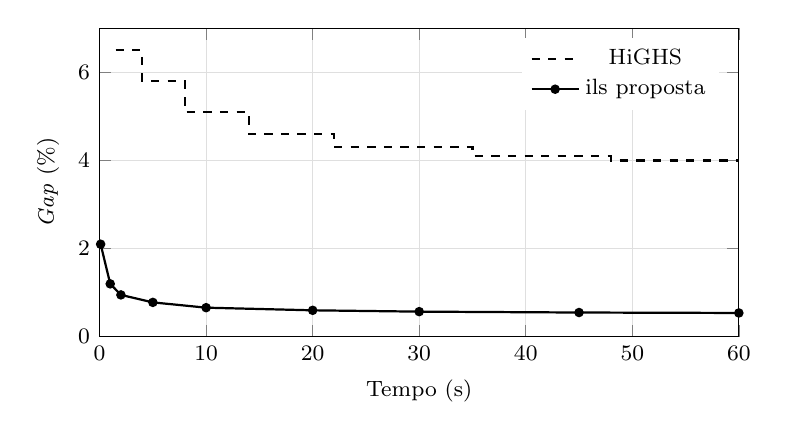
\begin{tikzpicture}
    \begin{axis}[
        width=0.8\textwidth, height=5.5cm,
        xlabel={Tempo (s)}, ylabel={\emph{Gap} (\%)},
        xmin=0, xmax=60, ymin=0, ymax=7,
        grid=major, grid style={gray!25},
        legend style={draw=none, font=\footnotesize},
        legend pos=north east,
        tick label style={font=\footnotesize},
        label style={font=\footnotesize},
      ]
      \addplot[const plot, thick, black, dashed] coordinates {
        (1.5,6.5) (4,5.8) (8,5.1) (14,4.6) (22,4.3) (35,4.1) (48,4.0) (60,3.95)
      };
      \addlegendentry{HiGHS}
      \addplot[thick, black, mark=*, mark size=1.3pt] coordinates {
        (0.1,2.1) (1,1.2) (2,0.95) (5,0.78) (10,0.66) (20,0.60) (30,0.57) (45,0.55) (60,0.54)
      };
      \addlegendentry{\acs{ils} proposta}
    \end{axis}
  \end{tikzpicture}
  \fonteautor
\end{figure}

\begin{instrucao}
\orientacao{Gráficos}
Há duas boas formas de produzir gráficos vetoriais. A primeira é desenhá-los
no próprio LaTeX com o pacote \verb|pgfplots|, como na
\cref{fig:convergencia}. Os dados podem vir de um arquivo CSV com
\verb|\addplot table[x=tempo, y=gap] {dados.csv};|. A segunda é gerá-los em
Python e salvar em PDF, como na \cref{fig:ablacao}, cujo script está em
\verb|figuras/cientifico/gerar_boxplot_ablacao.py|. Em ambos os casos:
\begin{itemize}
  \item nomeie os eixos e indique as unidades;
  \item use vírgula decimal nos rótulos (o modelo já configura o
        \verb|pgfplots| para isso e o script mostra como fazer no Python);
  \item diferencie as séries também por tipo de linha, marcador ou hachura, e
        não só pela cor;
  \item evite títulos dentro do gráfico, porque o título vai na legenda.
\end{itemize}
\end{instrucao}

% ------------------------------------------------------------------------------
\section{Contribuição da perturbação adaptativa}
\label{sec:experimentos:componentes}

Para avaliar o efeito da perturbação adaptativa, a heurística foi executada
também com perturbação de intensidade fixa ($k = 5$, o valor de melhor
desempenho nos testes preliminares). A \cref{fig:ablacao} compara as duas
versões nas instâncias com 500 itens. A versão adaptativa obteve \emph{gap}
menor nos três grupos e a diferença aumenta com o número de restrições. Esse
comportamento é coerente com o mecanismo da perturbação adaptativa. Em
instâncias mais restritas, a busca local fica presa com mais frequência.
Aumentar gradualmente a perturbação permite escapar desses ótimos sem
descartar a estrutura da solução corrente.

\begin{figure}[htbp]
  \centering
  \caption{\emph{Gap} das versões com perturbação fixa e adaptativa nas
    instâncias com 500 itens}
  \label{fig:ablacao}
  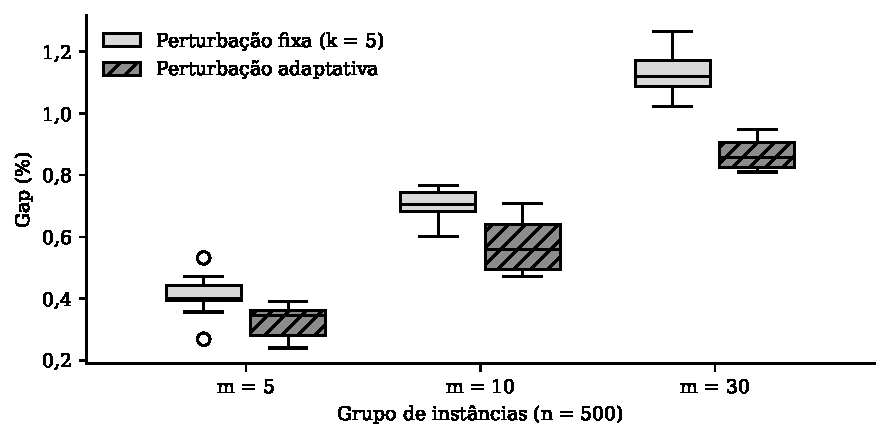
\includegraphics[width=0.85\textwidth]{figuras/cientifico/boxplot-ablacao.pdf}
  \fonteautor
\end{figure}

% ------------------------------------------------------------------------------
\section{Discussão}
\label{sec:experimentos:discussao}

Os resultados respondem afirmativamente à questão de pesquisa apresentada na
\cref{sec:introducao:problema}. Com 60 segundos, a heurística obteve soluções
mais próximas das melhores conhecidas do que o HiGHS em instâncias com 250 e
500 itens. Nas instâncias pequenas, o solucionador continua sendo a melhor
opção. Uma estratégia prática seria usá-lo quando o número de itens for
pequeno e recorrer à heurística nos demais casos.

Em relação ao \acs{ag} de \textcite{chu1998genetic}, a heurística obteve
resultados melhores com menos parâmetros. Os resultados, porém, ainda ficam
abaixo dos métodos híbridos, como o de \textcite{vasquez2001hybrid}, que
usam tempos de execução muito maiores.

Alguns fatores limitam a validade das conclusões. Os resultados do \acs{ag}
foram obtidos da literatura, em hardware diferente. Por isso, a comparação de
tempos entre os dois métodos é apenas aproximada. Além disso, os parâmetros da
heurística foram calibrados nas mesmas classes de instâncias usadas na
avaliação, ainda que com instâncias diferentes, o que pode favorecer o método
proposto nessas classes.

\begin{instrucao}
\orientacao{Ameaças à validade}
Discutir as limitações dos experimentos não enfraquece o trabalho. Pelo
contrário, mostra maturidade científica e antecipa perguntas da banca. Pense
em vieses nos dados, em comparações desiguais (hardware, tempo, implementação)
e em quanto os resultados podem ser generalizados para outros cenários.
\end{instrucao}
